%
% File acl2019.tex
%
%% Based on the style files for ACL 2018, NAACL 2018/19, which were
%% Based on the style files for ACL-2015, with some improvements
%%  taken from the NAACL-2016 style
%% Based on the style files for ACL-2014, which were, in turn,
%% based on ACL-2013, ACL-2012, ACL-2011, ACL-2010, ACL-IJCNLP-2009,
%% EACL-2009, IJCNLP-2008...
%% Based on the style files for EACL 2006 by 
%%e.agirre@ehu.es or Sergi.Balari@uab.es
%% and that of ACL 08 by Joakim Nivre and Noah Smith

\documentclass[11pt,a4paper]{article}
\usepackage[hyperref]{acl2019}
\usepackage{times}
\usepackage{latexsym}
\usepackage{graphicx}

\usepackage{url}

\aclfinalcopy % Uncomment this line for the final submission
%\def\aclpaperid{***} %  Enter the acl Paper ID here

%\setlength\titlebox{5cm}
% You can expand the titlebox if you need extra space
% to show all the authors. Please do not make the titlebox
% smaller than 5cm (the original size); we will check this
% in the camera-ready version and ask you to change it back.

\newcommand\BibTeX{B\textsc{ib}\TeX}

\definecolor{Orange}{RGB}{255,140,0}
\newcommand{\ek}[1]{\textcolor{Orange}{[ek: #1]}} 

\title{Predicting guilt judgments from crime stories}

\author{Elisa Kreiss \\
  Department of Linguistics \\
  Stanford University \\
  \texttt{ekreiss@stanford.edu} \\\And
  Judith Degen \\
  Department of Linguistics \\
  Stanford University \\
  \texttt{jdegen@stanford.edu} \\\And
  Christopher Potts \\
  Department of Linguistics \\
  Stanford University \\
  \texttt{cpotts@stanford.edu}\\}

\date{}

\begin{document}
\maketitle
\begin{abstract}
  \ek{update abstract wrt new framing}
  News has become a central part of our lives and with it our assessments and reproductions of these stories. However, the way in which humans assess guilt on the basis of such crime stories is unclear. If neural networks can learn to predict guilt judgments from a news story, they can help us form hypotheses about relevant features for human guilt predictions. However, whether neural networks can even learn to predict guilt judgments from a given news story is still an open question. In this paper, we will present a bidirectional LSTM with self-attention that makes a promising first step to predict guilt judgments. On the basis of attention visualizations, we argue that the model learns meaningful patterns from the data that guides its prediction.
\end{abstract}

\section{Introduction}

\ek{update according to framing proposal in email}

Deep learning models are increasingly applied to language tasks not only to develop technologies but also to derive new insights about language.

However, deriving scientific insights presupposes that the networks are learning sensible representations, which is often in question. Attention mechanisms have improved model performance and also made our networks more interpretable.

In this paper, we apply neural networks with attention to a task that has both linguistic and societal import: predicting whether the reader of a narrative text about a crime will conclude that its main subject is guilty or innocent.

Our models are good at this task, which is nice. However, we are, in particular, interested in seeing how our networks attend to markers of certainty and uncertainty in these texts. To what extent do these epistemic markers guide network decisions?


% In the current world we are constantly confronted with news. We consume it by reading the newspaper, listening to news channels, but also through social interactions, for example conversations with friends. 
% A crucial aspect of news is the uncertainty that comes with different stories. For example news can report on advances in crime investigations that are still in progress, such as the arrest of a suspect. Most importantly, an arrest does not imply that the suspect is in fact guilty or even that the investigation is completed. Reporting is often not simply about guilty or not guilty, but a graded notion of guilt presenting a range of evidence from definite to only suggestive.

% After observing the news, they are retold and passed on through social interactions. It is essential that the uncertainty which was previously communicated, will propagate to the next person we tell the story to. This person in turn can tell the story to someone and so on. If we had perfect memory, reproduced stories would be exact replica of their predecessors. However, reproduction is not only a lossy but also faulty process. \cite{Bartlett:1932} introduced this transmission chain paradigm as a scientific method and showed not only that information get lost, but also that they get distorted. Subsequent work found that the person's priors and beliefs shape their reproductions of stories \citep{Allport:1945,Kashima:2000,Griffiths:2007}. In other words, people's initial guilt assessments after hearing a story will affect how they will reproduce it. It is therefore relevant which guilt judgments people form and what these are influenced by.

% However, guilt judgments are very complex. Assessing the likelihood of someone's guilt could be dependent on how persuasive we find their alibi, how condemning their motive appears and even prejudices against race or culture of the suspect could play a role. Additionally, the presentation of the news seems relevant: How detailed is the report? Does the story serve the ideological purposes of the person reporting on it? 

% There are many more of these potential aspects that we can reasonably assume to affect our guilt judgments. In other words, there are numerous potential features that could affect our guilt perception when assessing a crime story. This complexity provides a big challenge to our investigation of what guides these guilt judgments. Testing all of these potential factors randomly is highly inefficient. Ideally, we would like to form hypotheses about promising aspects with respect to the language used in the text. Those can then be tested in controlled human subject experiments to inform our theory about guilt perception.

% But which resources can we employ to inform us about promising hypotheses? One approach might be to ask participants directly about their reasons to find a suspect more or less guilty. However, these \ek{self reports} can be highly biased. For example, \ek{people have a tendency to rationalize their racial biases (cite "the limitations of implicit bias"); implicit biases (jennifer eberhardt, perdy 2004); basis for manipulation is unconscious and therefore non-reportable}

% Can neural networks be tools to inform hypotheses about human guilt judgments? Since neural networks try to approximate a complex function, their prediction is simply data driven and their evaluation will not be distorted by the biased human self reports. Furthermore, it has the potential to detect patterns that might influence us without our awareness. Therefore, neural networks are a promising method to inform hypotheses about relevant features that influence human guilt judgments.

% However, these considerations assume that a neural network can find meaningful patterns in the data which predict guilt judgments. But is that the case? Can neural network models learn to predict human guilt judgments? In this work, we investigate whether a bidirectional LSTM with attention can model empirically collected guilt ratings of propagated news stories. Crucially, these stories are very similar in content and still show remarkable variations in the guilt judgments people draw. Can a model pick up on these small differences and on their basis make meaningful inferences about guilt perceptions?

% We argue that neural network models are capable to predict human guilt judgments on the basis of news articles. Furthermore we argue that they learn meaningful patterns in the data that we can nourish. We show that simple neural network visualizations as well as inspecting guilt predictions while making controlled and systematic changes to the stories are promising ways to probe the inner workings of the model.

\subsection{Related work}

The central challenge is to find a promising neural network architecture that can extract relevant features of an input paragraph. This can then be used to predict a value that represents a guilt judgment.

\paragraph{Word embeddings}
There are a variety of systems that investigate how to find meaningful word representations. In the literature, GloVe word embeddings \citep{Pennington:2014} have been widely used to represent word meanings. Those embeddings are context-independent, i.e., each word only has one respective vector representation independent of the context it occurs in.

More recent advances in word embeddings aim to provide context-sensitive word representations to obtain richer and more informative word meaning representations (e.g., ELMo \cite{Peters:2018} and BERT \cite{Devlin:2018}). The BERT word embedding model is a Transformer based network which incorporates the context before and after the critical word to obtain a word representation. \citeauthor{Devlin:2018} report that using these embeddings boosts performance in all of the 11 natural language tasks it was trained on compared to previous systems.

\paragraph{Paragraph embeddings}
While word embeddings are useful, we need to arrive at a meaningful \textbf{paragraph} representation for our purposes. In other words, the word embeddings need to be combined in a meaningful way to arrive at a more complex representation.

For short phrases, bidirectional LSTMs \cite{Hochreiter:1997,Schuster:1997,Graves:2005} have been shown to be a useful tool. However, they have difficulty resolving long-term dependencies, which is why their performance decreases with longer input paragraphs \cite{Hochreiter:2001}. \cite{Vaswani:2017} developed am attention mechanism to resolve these issues in Transformers. However, a similar principle can be applied to LSTM architectures as well.

\cite{Lin:2017} introduce a bidirectional LSTM with self-attention that receives word embeddings as an input and outputs a paragraph representation. The bidirectional LSTM receives the GloVe embeddings of the paragraph as input. The self-attention layer is the weighted sum of all of the LSTM's hidden states. But instead of using a single weighted sum to arrive at a vector, they suggest to perform this multiple times with different weight vectors to arrive at an attention matrix. Furthermore, they introduce a penalization term which ensures that each attention vector in this attention matrix focuses on different semantic features of the input paragraph. Which semantic features are more important than others can in turn be learned again, dependent on the task it needs to solve. \citeauthor{Lin:2017} report that the model outperforms previous models in author profiling, sentiment classification and textual entailment.

\section{Dataset}
For training and testing the model, we use the Annotated Iterated Narration Corpus (AINC) collected by \cite{Kreiss:2019}. The corpus was created for investigations on how news stories change when they are propagated from one person to another. First the authors created five stories of approximately 850 words, which are called the \textit{seed} stories. All of them report a crime and an arrest of one or more suspects. Each of these five seed stories exists in a weak and a strong evidence condition. The stories are identical up to the last phrase which then either raises doubts about the arrest or emphasizes its validity. For example, if a suspect was arrested on the basis of camera footage, this footage was described as being of ``very poor quality" in the weak evidence condition and ``very high quality" in the strong evidence condition. Each story was given to a participant who was asked to read and afterwards reproduce it. The reproduced story was then given to the next participant who again reproduced it. This pattern was repeated for 5 generations of participants. The data collection therefore followed the transmission chain paradigm, introduced by \cite{Bartlett:1932}. Following this schema, each story and condition was reproduced in 5 chains over 5 generations, resulting in 250 reproductions, and therefore 260 stories overall (see Figure \ref{fig:corpus-overview}).

\begin{figure}[t!]
	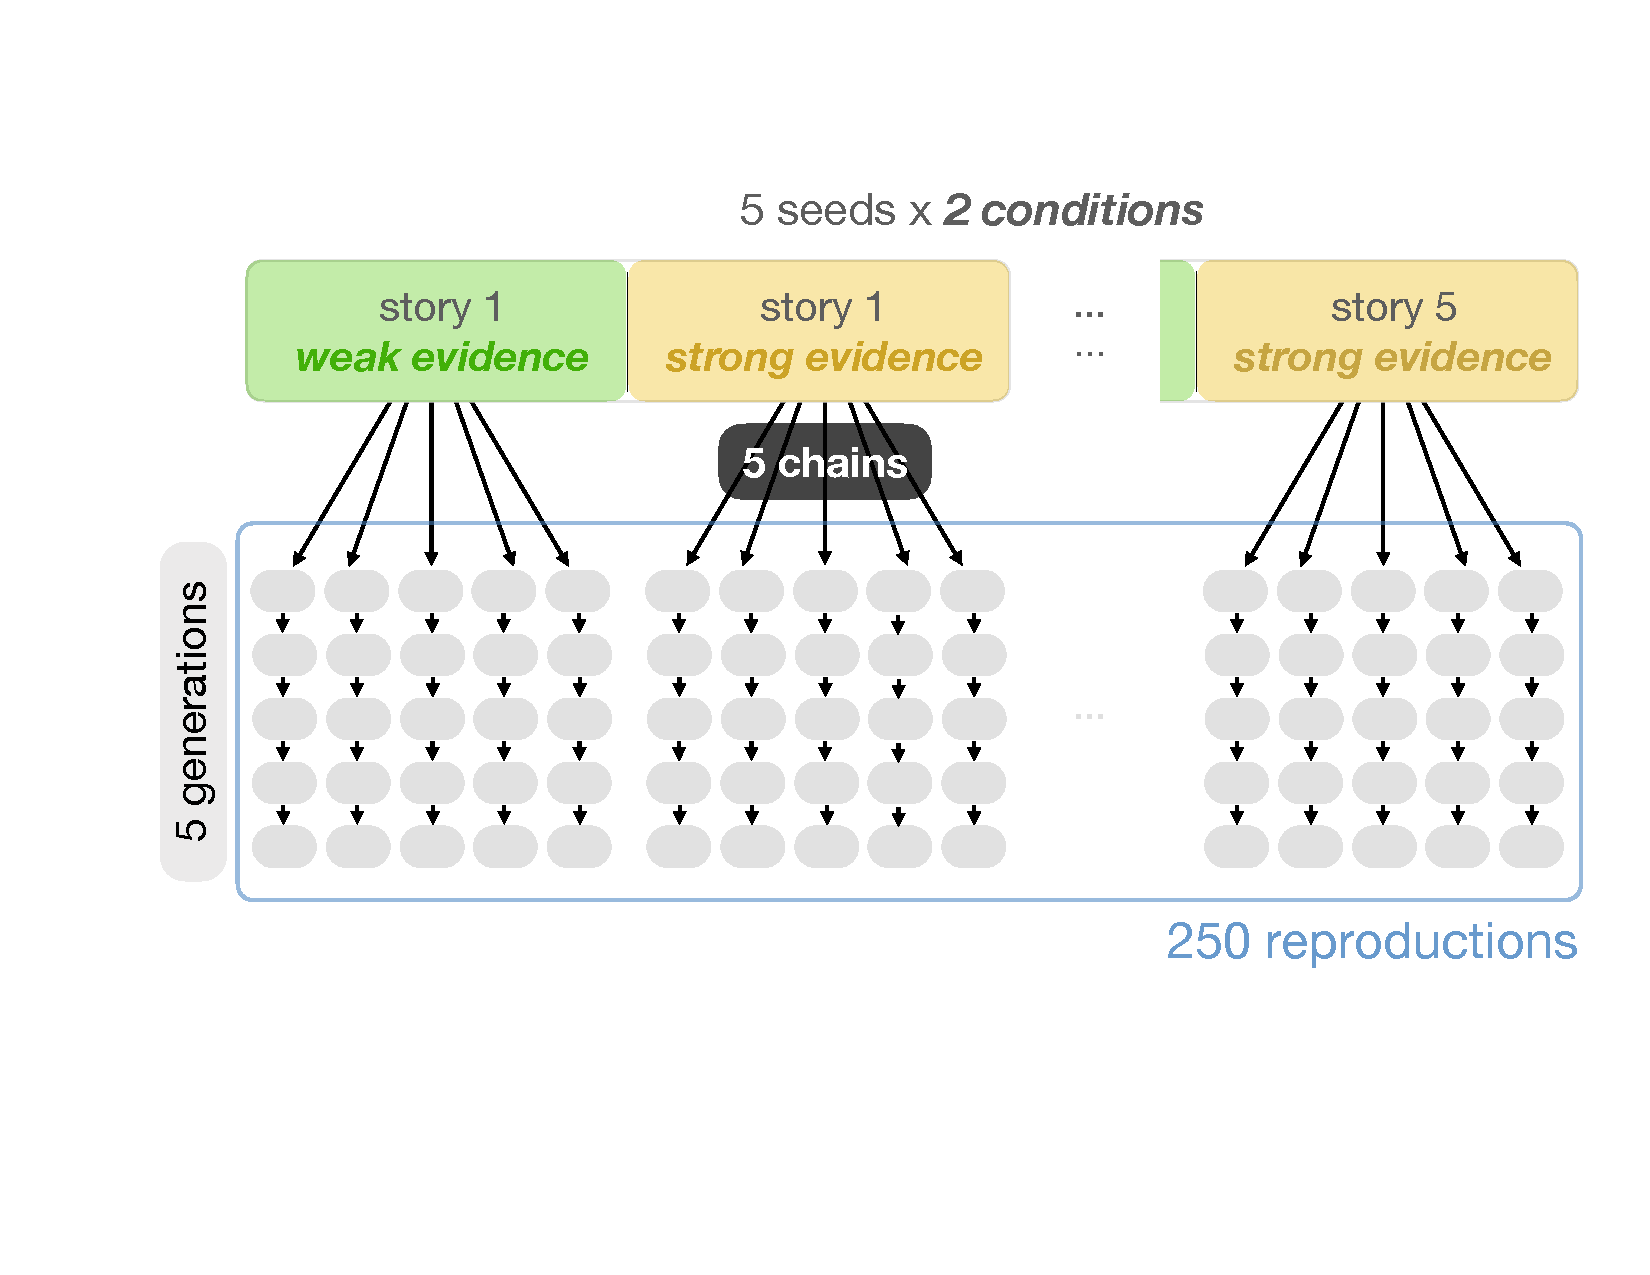
\includegraphics[width=\linewidth]{graphs/corpus-overview.pdf}
	\caption{Corpus collection schema as presented in \cite{Kreiss:2019}.}
	\label{fig:corpus-overview}
\end{figure}

After the corpus collection, \citeauthor{Kreiss:2019} annotated the corpus with human judgments. The questions were primarily related to different aspects of guilt perception but also for example perceived subjectivity of the story writing. Participants were recruited on Amazon Mechanical Turk and indicated their response on a continuous slider, here underlyingly coded as ranging from 0 to 1. Most interestingly for this project, they asked ``How likely is it that the suspect is / the suspects in the crime are guilty?". Each story received approximately 20 ratings, ranging from 0 to 1. For the purpose of this work, we will consider the mean rating for each story as its guilt judgment label. The labels of each story are shown in Figure \ref{fig:corpus-annotations}. In contrast to the raw ratings, the means only range from 0.27 to 0.92. 

% Subsequent analyses revealed that there are correlations with the number of hedges in the story, the length of the stories and of course with the evidence condition and therefore content expressed. 

\begin{figure}[t!]
	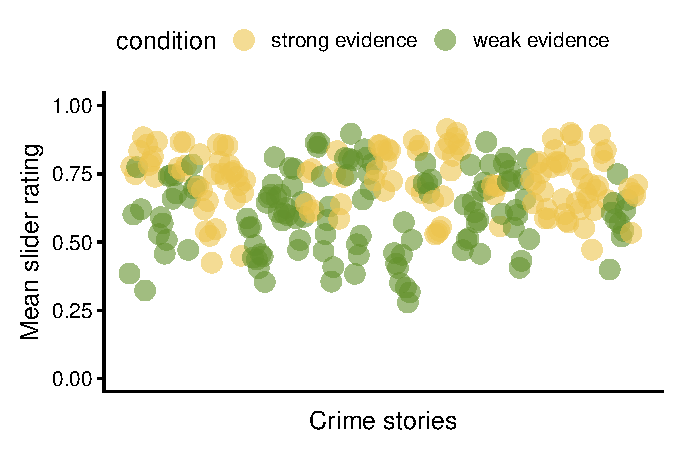
\includegraphics[width=\linewidth]{graphs/subjguilt.pdf}
	\caption{A point represents the mean subject guilt rating for a story in the corpus. They are color-coded with respect to their condition.}
	\label{fig:corpus-annotations}
\end{figure}

In summary, the AINC is a corpus of reproduced news stories, annotated by human guilt judgments. Since the stories originated from only 5 unique stories (each in 2 conditions), a lot of information is shared between single data points.  Despite this similarity, the range of guilt judgments is still high, alluding to subtle differences that trigger this variance. 
One of the challenges, this dataset poses, is its size. There are only 260 labeled examples that can be used for training and testing a model.
Can a bidirectional LSTM with attention pick up on the patterns in human judgments with only very limited available data?

\section{Model}

The goal of this work was to determine whether neural networks can be a useful tool to investigate the formation of guilt judgments. To do this, we used a model which was based on the design proposed by \citeauthor{Lin:2017}. We chose to use this model as our base because of its promising performances in various NLP tasks. Furthermore, its attention module provides a straightforward way to investigate the inner workings of the model. 

We made two major adjustments to the model proposed by \citeauthor{Lin:2017}. Firstly, we simplified the attention module to represent a vector and not a matrix. Second of all, we replaced the GloVe word embeddings by BERT embeddings\footnote{In their paper, \citeauthor{Devlin:2018} showed that BERT embeddings (can) improve existing NLP systems. Pilot runs in the development of the model showed that BERT improved the convergence of the model.}.

The following sections will explain the model architecture and the training of the model in detail.

\subsection{Architecture}
\label{model-architecture}
The tested model (see Figure \ref{fig:model}) receives a crime story as an input and outputs a value between 0 and 1. This value is interpreted as a continuous guilt assessment of the suspect in the story.

\begin{figure}
	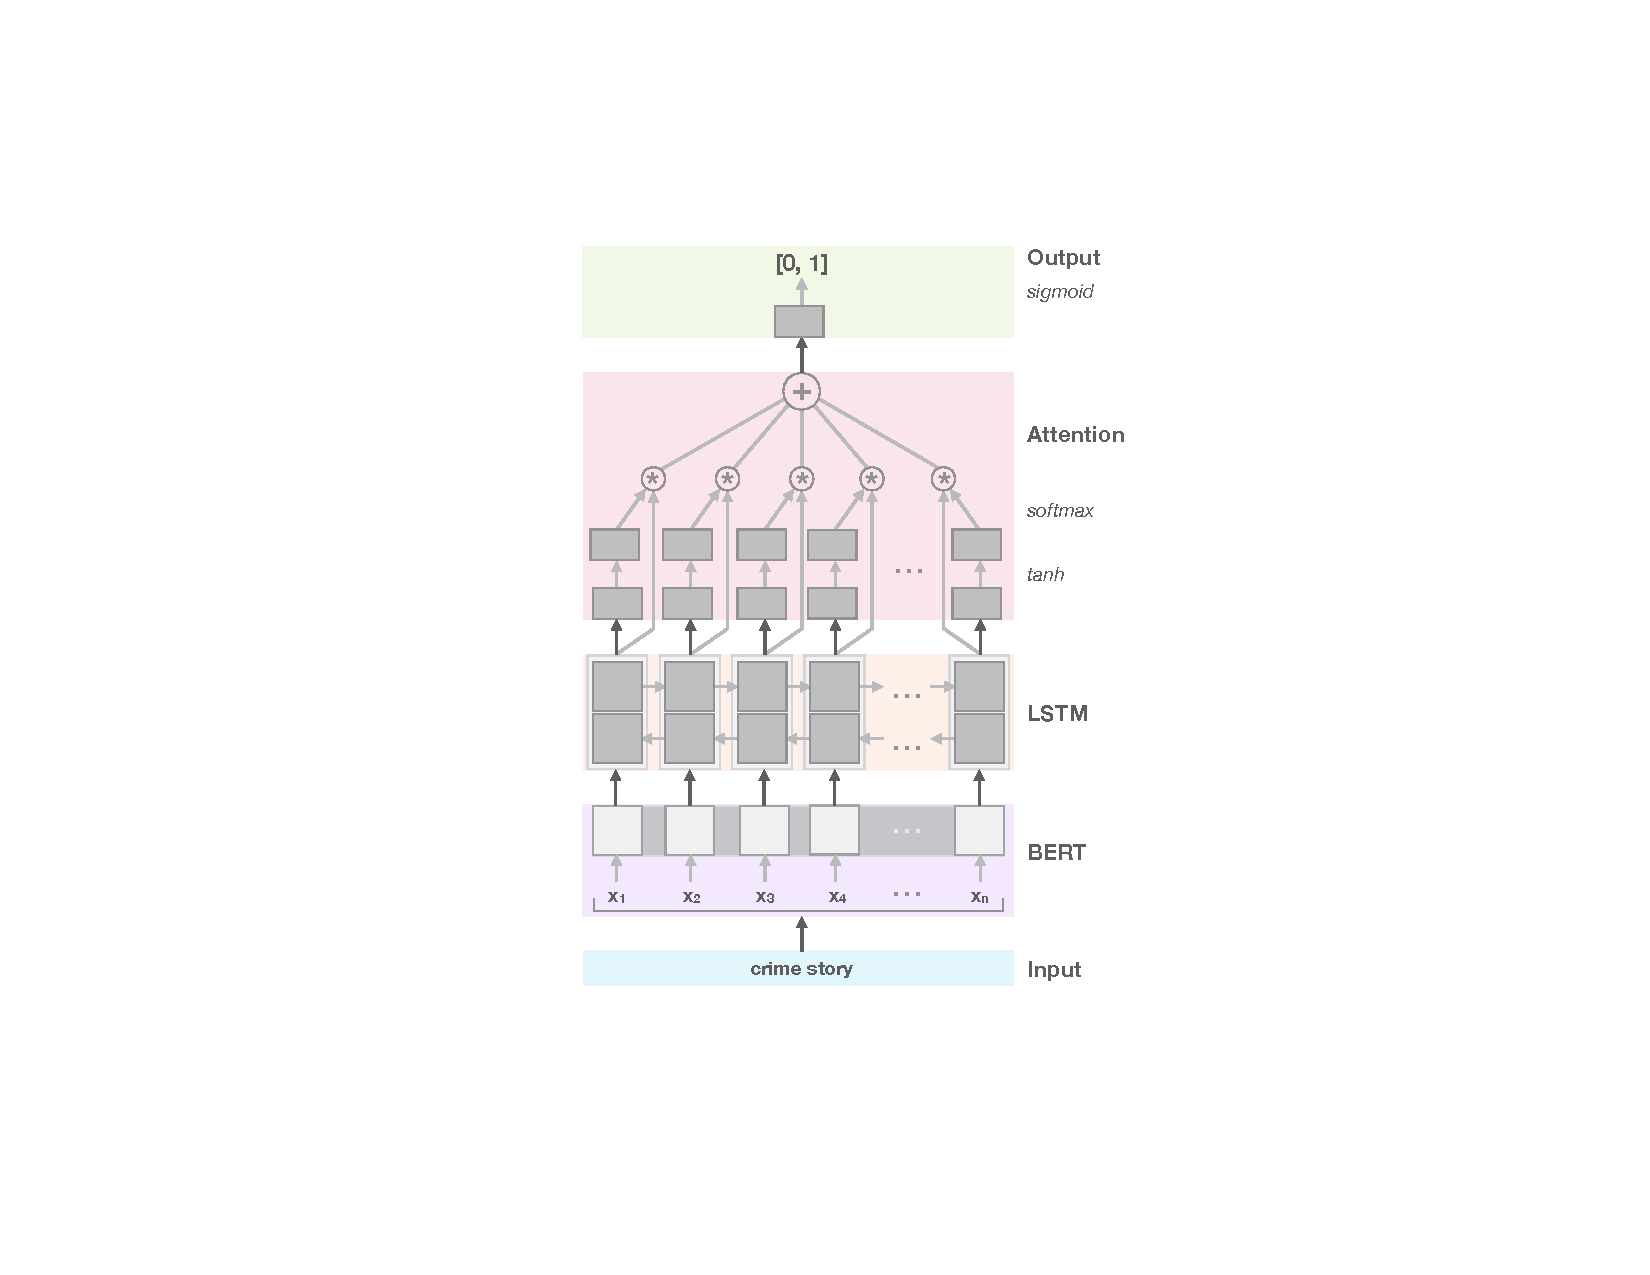
\includegraphics[width=\linewidth]{graphs/model.pdf}
	\caption{Proposed model architecture to predict guilt judgments (between 0 and 1) from news stories. The arrows indicate the information flow. The boxes stand for operations performed on the data.}
	\label{fig:model}
\end{figure}

Overall, the model consists of four main modules (see Figure \ref{fig:model}). First the crime story is transformed into \textbf{word embeddings}. These are the input to a bidirectional \textbf{LSTM} with \textbf{attention}, which will output a single vector representation for the whole input sequence. To obtain the desired output in the range [0, 1], a simple \textbf{logistic regression} is performed on the vector. 


\paragraph{Word embeddings (BERT)}
We used a pretrained BERT model as the word embedding module (represented by the yellow box in Figure \ref{fig:model}). The module receives the original crime story as an input and returns a word embedding for each token in the story $(x_1, x_2, ..., x_n)$. For tokenization, we used the BertTokenizer implementation in the python package 
\textit{pytorch-pretrained-bert}
\footnote{Huggingface Inc., https:\slash \slash github.com\slash huggingface\slash pytorch-pretrained-BERT, June 09 2019}. 
The BERT word embeddings for each token were extracted from the Google-pretrained base BERT word embeddings (uncased) with 768 hidden layers. Note that given the requirements of the pretrained BERT model, the original story had been transformed to all lower-case letters.

This module takes the raw crime story as input and returns a word embedding representation for each of the $n$ tokens in the text. The output is therefore of size $n \times 768$.

\paragraph{LSTM}
The bidirectional LSTM (represented by the orange box in Figure \ref{fig:model}) takes the word embeddings as input to enhance the contextual representation of the story.
% \begin{math}
% 	\overrightarrow{h_t} = \overrightarrow{LSTM}(x_t, \overrightarrow{h_{t-1}})
% \end{math}

% \begin{math}
% 	\overleftarrow{h_t} = \overleftarrow{LSTM}(x_t, \overleftarrow{h_{t-1}})
% \end{math}\\
The LSTM has 200 hidden dimensions. Since a bidirectional LSTM concatenates the hidden states of the forward and backward LSTM, each hidden layer has 400 hidden dimensions. 
% $H = (\mathbf{h_1}, \mathbf{h_2}, ..., \mathbf{h_n})$\\
Therefore, the LSTM module receives an input of size $n \times 768$ and returns a matrix $H$ of size $n \times 400$.

\paragraph{Attention}
The attention module (represented by the red box in Figure \ref{fig:model}) creates a weight for each input token before they are summed over. The boxes inside the attention module stand for linear operations that reduce the dimensionality of the input. Tanh and softmax are non-linear transformations on the output of these dense layers.

The LSTM module returns $H$, i.e., $n$ hidden states of size 400. These are first linearly reduced to $n \times 50$ dimensions and tanh transformed. 

$A_1 = tanh(W_{a1} H)$\ek{Lin has here $H^T$, but this is not true for our model}\\
The resulting matrix $A_1$ is further compressed to the attention weight vector $\mathbf{a_w}$ of size $n \times 1$. The softmax ensures that its values sum to 1.

$\mathbf{a_w} = softmax(\mathbf{w_{aw}} A_1)$

Now we take the dot product of the LSTM hidden state matrix $H$ and the just obtained vector $a_w$ to obtain the attention output vector $\mathbf{a_{out}}$ of size $400$. 

$\mathbf{a_{out}} = a_w^T H$\\
This is the output of the attention module.

\paragraph{Output (Logistic regression)}
The logistic regression module is represented by a blue box in Figure \ref{fig:model}.
For a prediction, the output of the attention module ($\mathbf{a_{out}}$) is linearly transformed into a single number. 
% $p = sigmoid(\mathbf{a_{out}})$\\
The Sigmoid function ensures that the prediction lies between 0 and 1, just like the restriction on the guilt judgments it is trained on. 


Overall, the model has 111,054,742 trainable parameters. Only 0.02\% of them are in the attention and output modules, and 1.40\% are in the LSTM module. These parameters were initialized randomly. The rest of the parameters (98.59\%) are the pretrained weights in the BERT word embedding module.

In summary, the model receives a crime story as an input. BERT word embeddings for the story feed into a bidirectional LSTM. The attention module computes the weighted sum over the LSTM's hidden states. The resulting attention vector is fed through a linear layer and a Sigmoid function to ensure that the prediction lies between 0 and 1.

\subsection{Training}

To begin with, we randomly held back 26 stories (from the 260 stories in total) as the final test set. This helps to assess the model performance on a set of stories which has never been evaluated in the process of model development. The remaining 234 stories were then for used for model training and validation, which was done using 10-fold cross validation. The cross-validation results inform us about the model variation given various training/validation splits. For example, it is quite likely that given the small size of the dataset, this variation could be quite high. Note that, each fold had either 23 or 24 stories in it, each of which was associated with a guilt rating that functioned as the target label. Recall that this guilt rating is the mean subject guilt rating obtained from the previously described data collection and annotation. 



%From the 260 stories with their respective mean suspect guilt rating, 26 were randomly held back as a final testing set. The guilt rating is the mean obtained from the previously described data collection and annotation. Crucially, the target values range between 0 and 1, which is why the model does not learn a classification, but regression task. The remaining 234 stories were used for training the model. 

%To assess the model performance during development, we need to exclude more stories from training to be able to use them as dev-testing data. To make the most use of the limited amount of data, the model was trained using 10-fold cross-validation. The results can also inform us, whether there is strong variation given a different training/dev-testing split. It is very likely that given the small size of the dataset (and therefore dev-test set), the variation can be quite high. Given that there were 234 stories for training, each fold had between 23 and 24 stories, each associated with one guilt rating that functioned as the target label. 

For training, the model uses mean squared error (MSE) as the loss function, stochastic gradient descent as the optimizer and a learning rate of 0.1. The whole model was implemented using pytorch \citep{Paszke:2017}. It was trained for 30 epochs, for each of the 10 training/dev-test configurations in the cross-validation.

\section{Experiment}

This work investigates whether a bidirectional LSTM with self-attention (as described in Section \ref{model-architecture}) can predict human guilt judgments from news stories. In each step of the 10-fold cross-validation, the model was trained on 206/207 stories and 23/24 were held out for dev-testing. Each story has an associated suspect guilt rating, which is the mean rating obtained from human judgments. This value functions as the target label.

Since the target labels only range between 0.27 and 0.92, one potential problem might be that the model only learns to predict the overall mean of the labels in the training data. We would also expect this outcome if the model does not find any features that it can take as predictors for guilt ratings. This is why, the baseline model to test the dev-test data on will simply predict the mean of the training data labels. If the our model outperforms this baseline, we will consider it worthy of further investigations.

Both model performances will be evaluated on the mean-squared error (MSE) of their prediction to the target label on the cross-validation test set.

\subsection{Results}

\begin{figure*}
	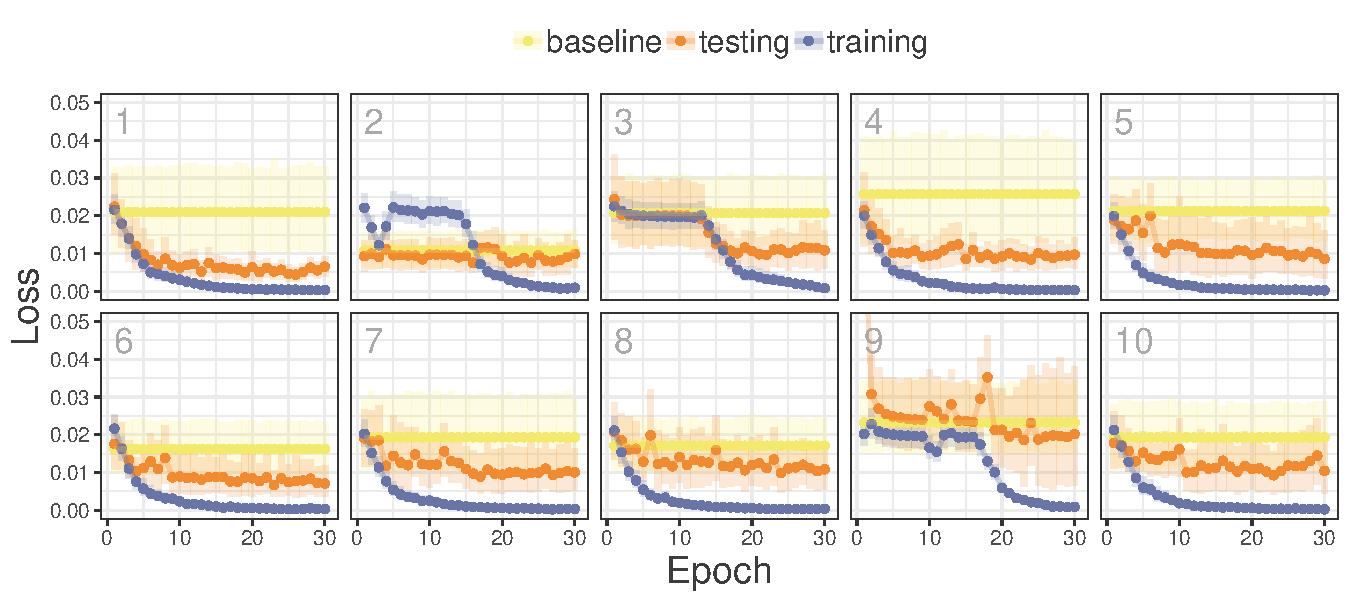
\includegraphics[width=\linewidth]{graphs/lossPlotCropped.pdf}
	\caption{Loss (mean squared error) over epochs (x axis), faceted over cross-validation configurations. The performance of the model on the training set (in blue) approaches zero. The performance of the model on the dev-test set (in orange) generally outperforms the baseline (in yellow).}
	\label{fig:loss}
\end{figure*}

Figure \ref{fig:loss} shows the mean squared error (MSE) loss for each training epoch. Firstly, the training loss (in blue) is approaching a loss of 0 toward the end of the training in all cross-validation configurations. Thus the amount of training epochs seems to be sufficient. Crucially, the dev-testing loss (in orange) is overall lower after the last training epoch than the baseline (in yellow). Therefore, the model obtains information from the dataset that it can use to improve its predictions. However, there is also a high amount of variation between the different cross-validation steps. The mean of the training labels alone (i.e., the baseline) only has a very small loss on cross-validation configuration 2 and the trained model can barely beat it. This is in clear contrast to cross-validation step 4, where the baseline model loss is very high on the dev-test data and the trained model can easily surpass it. Those two cases exemplify the high variation that comes with the different splits of training and dev-testing data\footnote{However, I cannot exclude that also the random parameter initialization plays a relevant role here. But at least the differences in the baseline are definitely caused by the different splits.}.

But looking at the MSE loss alone is not on its own sufficiently informative to assess how well the model actually learns to predict the underlying distribution. Figure \ref{fig:corr-cv0} shows the correlation between the actual target label (on the x axis) and the model prediction (on the y axis) for cross-validation step 0. Before training, the training and dev-testing data has a high variance around the perfect correlation line ($r=1$). The model only predicts values between 0.48 and 0.79. However, the underlying labels range from 0.31 to 0.92. Even though the Pearson correlation still predicts a rather high correlation on the testing set ($r=0.65$), the mean squared error is comparably high with $0.022$. 

Already qualitatively, the model predictions after training (Figure \ref{fig:corr-cv0}) seem far more informative. Now the model predictions have approximately the same range as the target labels (between 0.33 and 0.91). The Pearson correlation itself is now $0.85$, and the mean squared error reduced to $0.007$.

Since the baseline model does not learn over training epochs, its predictions stay the same.

\begin{figure}
	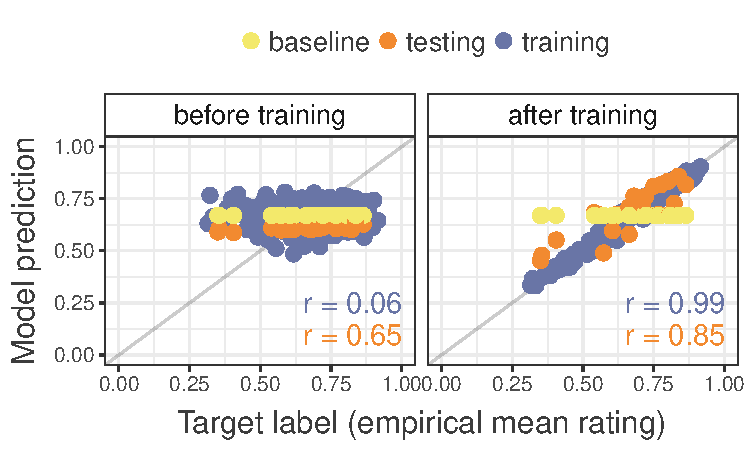
\includegraphics[width=\linewidth]{graphs/cv0-pred-target-epoch0-29.pdf}
	\caption{Correlation between target label (x axis) vs. model prediction (y axis) before and after training.}
	\label{fig:corr-cv0}
\end{figure}

Qualitatively, these plots appear very similar throughout all cross-validation configurations and can be compared in Figure \ref{fig:app-corr-pretraining} and \ref{fig:app-corr-posttraining} in the Appendix. However, quantitatively the correlation on the dev-test set changes. Those differences are mainly driven by outliers.

Overall, the mean correlation between the model prediction and the human judgment on the testing set across all cross-validation steps is $0.68$. When we collapse over all cross-validation folds and examine the loss after training, the difference in loss between the model predictions and baseline is significant ($p<0.0001$).

\label{model-results}

As a final performance evaluation, we can examine the target-prediction correlation on the held-out test set (see Figure \ref{fig:test-corr}). For predictions on the test set, we used the final model weights obtained by the first cross-validation configuration. This setup was chosen, because of the low dev-testing loss and the high correlation of the dev-test set with the target labels\footnote{This was the only evaluation that was performed on this held-out test set.}. 

The Pearson correlation on the held-out test set is still $0.84$ and almost identical with the performance on the dev-test set. This fairly high correlation and the fact that the high correlation reproduces with the held-out testing data indicates that the model learns something meaningful that can generalize well.

\begin{figure}
	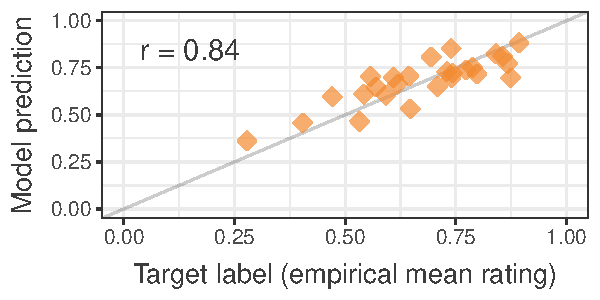
\includegraphics[width=\linewidth]{graphs/test-corr.pdf}
	\caption{Testing label (x axis) vs. model prediction (y axis) after training on the held out test set (26 data points) using the parameter settings obtained after the 30th epoch from the first cross-validation. Pearson correlation of 84\%.}
	\label{fig:test-corr}
\end{figure}

\section{Model analysis}

We have seen that the proposed model can predict human guilt judgments when given a crime story. However the question remains whether there are patterns that underlie these predictions and whether we can interpret them. This is especially necessary, if we want the model to inform hypotheses about the processes that possibly underlie human judgments.

\subsection{Visualization}

First, we need to investigate whether the model seems to pick up on patterns that are meaningful and possibly even interpretable for us.

In the original introduction of the attention mechanism, \citeauthor{Vaswani:2017} suggested that a visualization of the attention weights can inform us about what affects the network's prediction. We follow this approach to look for first indications of a meaningful representation in the $\mathbf{w_{aw}}$ attention weight vector described in Section \ref{model-architecture}. Since the softmax forces the sum of the weights to be 1, we cannot interpret the weights on their own for each word or across stories. Instead, the relevance lies in the differences between words and phrases within each story and pattern similarities between stories.

To investigate what might affect model predictions, we ran the model again on the final test data (as described in Section \ref{model-results}). Figure \ref{fig:viz} displays three of these stories with their attention weight distribution.

\begin{figure*}
	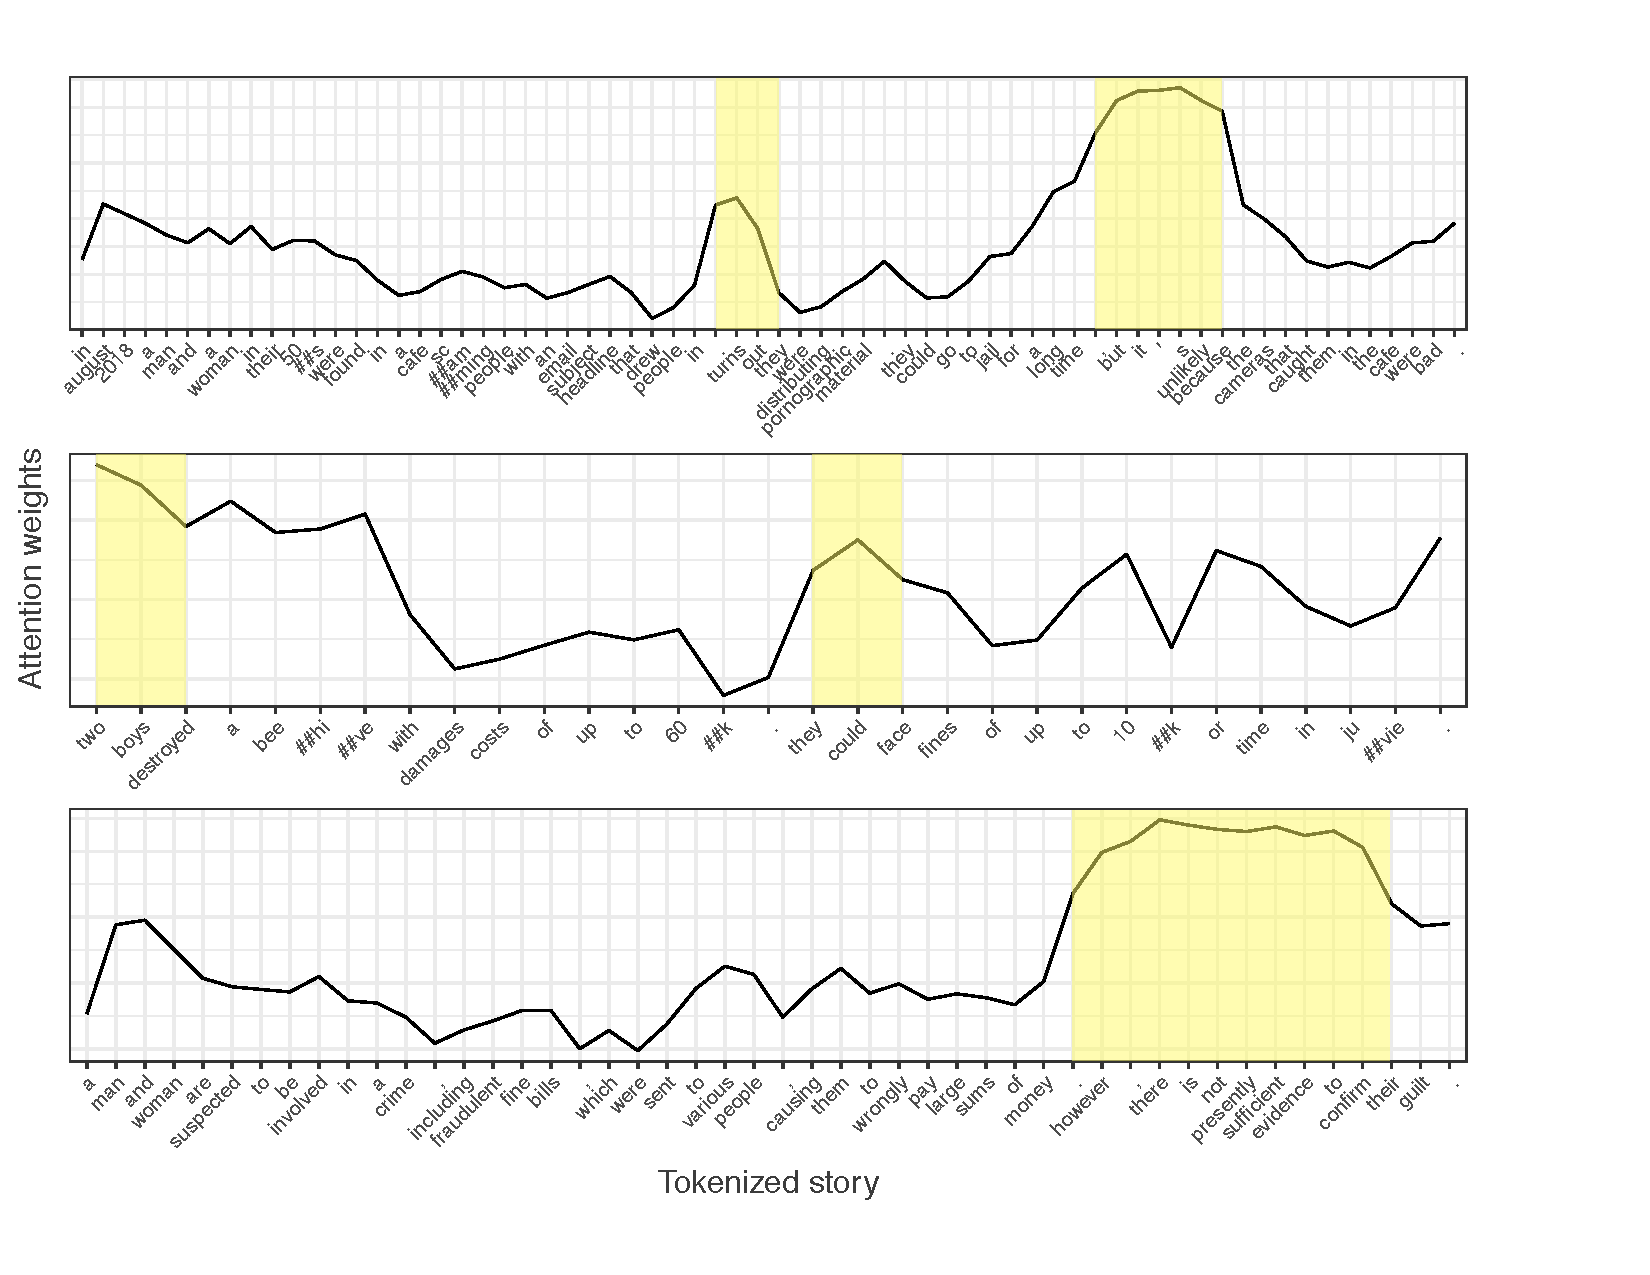
\includegraphics[width=\linewidth]{graphs/attention-marked.pdf}
	\caption{Visualization of the attention weights (y axis) for a tokenized story (x axis) from the test set. Because we took the softmax over the attention weights, the scale of the y axis is irrelevant. Interesting aspects are marked in yellow.}
	\label{fig:viz}
\end{figure*}

The model seems to focus on phrases that explicitly describe uncertainty about the evidence (see Figure \ref{fig:viz}C). If present, they usually outweigh the rest of the story. This suggests that if there is an explicit claim that affects the evidence of the suspect's guilt, it is considered as the most important source to inform guilt judgment.

Additionally, peaks occur on words and phrases which communicate turning points in a story, such as ``however", ``but", ``even though" and ``it turns out". This can be seen in all three stories in Figure \ref{fig:viz}. Those phrases could be relevant because they usually indicate a contrast to a prior narrative. Since those markers mostly follow reports of arrests, they might be strongly correlated with objections to those arrests which would in turn influence guilt perceptions.

Figure \ref{fig:viz}B shows a case where the model seems to find a simple declarative (``two boys destroyed") to be relevant for the final prediction. This is especially interesting, since declaratives on their own do not generally communicate guilt-related information. However, they are very important for guilt judgments because they do not allow any uncertainty about the association between crime and suspect.

In summary, the visualization of the attention weights contribute further evidence that the model learns meaningful patterns in the data.

\subsection{Qualitative analysis}

The model visualization provides evidence for the claim that the model picks up on meaningful patterns in the corpus. This allows us to use the model to inform new hypotheses.

But does the model make reasonable predictions on newly constructed data points?
The original corpus started out with five different crime stories. Each of these stories occurred in two conditions -- one suggesting that the evidence that led to the arrest was weak, and the other that the evidence provided a strong case. Additionally, the stories were filled with uncertainty markers such as ``allegedly" or ``(un)likely". The corpus cannot inform us about the relationship between those uncertainty markers and the evidential manipulation. What happens if we ask the model to predict a guilt judgment for each of the original stories without those uncertainty markers/hedges?

To investigate how hedging influences model predictions, we rewrote those 10 original stories into versions without any uncertainty markers. Note that they remained as close to the original as possible, while still remaining grammatical.

\begin{figure}
	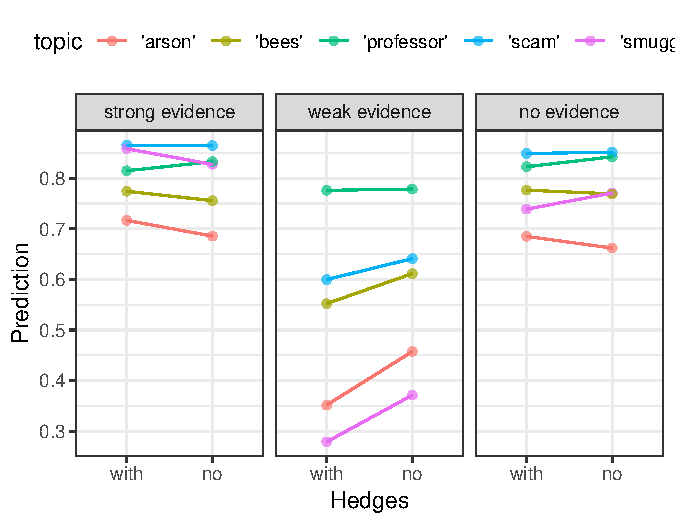
\includegraphics[width=\linewidth]{graphs/hedges.pdf}
	\caption{Model predictions on the relationship between uncertainty markers and evidence statements. \ek{fix caption and make figure more readable}}
	\label{fig:hedges}
\end{figure}

Figure \ref{fig:hedges} shows the results of this analysis. The results suggest that uncertainty markers have different effects on guilt prediction in the two evidence conditions. When the evidence is strong, removing all uncertainty markers does not affect the guilt judgments. However when the evidence is weak, removing those hedges increases the guilt judgment.

This allows for an intuitive interpretation. When evidence already overwhelmingly speaks for the suspect's guilt, it outweighs the hedges. However if the evidence is questionable, other sources of uncertainty are considered to inform a final judgment.

Notably if the evidence manipulation is excluded, the model predicts guilt judgments in the range of the strong evidence condition. In other words, the model predicts that a reassurance that the arrest is justified does not change the guilt judgments. However, formulating explicitly that there are reasons to question the arrest, causes the guilt assessments to drop.
When we remove the hedges again, we cannot see a common structure to the change in ratings (possibly more similar to the strong evidence ratings though).

\subsection{Conclusion}

In this section we showed that our attention module provides intuitive insight into the model workings. Furthermore, the model makes interesting predictions on new data.\ek{...}

\section{Discussion}

The results show that when given a news story, a bidirectional LSTM with self-attention can already capture something essential about human guilt judgments. Especially considering the limited amount of data (only 236 data points in the training set), the model can already extract meaningful features for guilt judgment predictions. 

So far, the model has not been subjected to hyperparameter tuning. It is likely that this will further boost the model's performance. Furthermore, it is plausible that training and testing the model on the guilt ratings directly instead of their means can further increase the performance, since only showing the means hides a vast amount of information about the underlying distribution of ratings which can be very meaningful. For example, a news story where participants highly vary in their judgments should influence the model predictions less than a story with low variance.

The introduced model is a promising first step to develop a better understanding of human guilt judgments. I am confident that in the future models like these can be used to inform hypotheses about what humans consider for their assessment. This can in turn inform us about how different reporting on a news story will influence these assessments.



\section*{Acknowledgments}

I'm particularly thankful for the valuable feedback from Sebastian Schuster. \ek{any grants to cite here, Judith?} \\

% \section*{Project authorship statement}

% This is an individual project and therefore, E. K. was responsible for all parts of the projects. 


\bibliography{acl2019}
\bibliographystyle{acl_natbib}

\onecolumn
\section{Appendices}
\label{sec:appendix}

\begin{figure*}[!htb]
	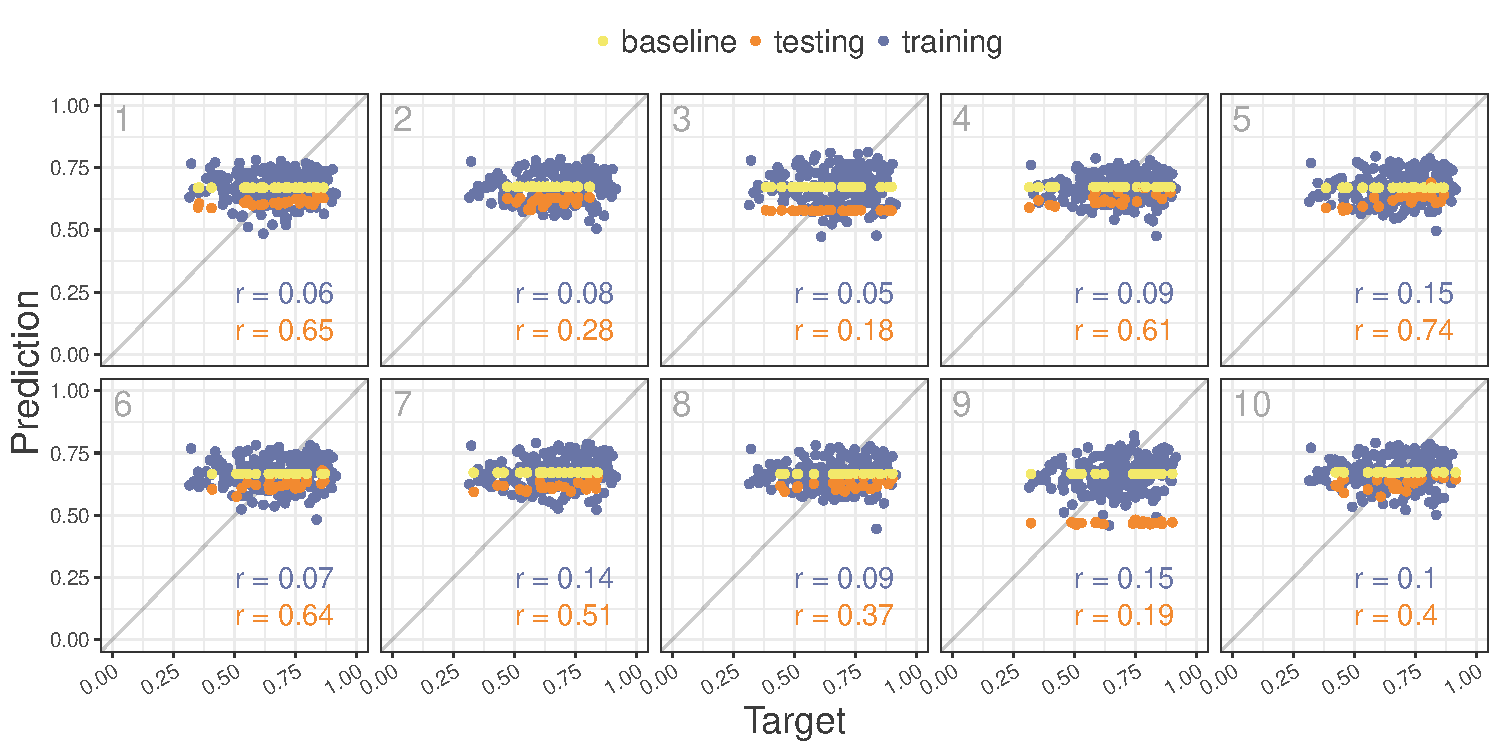
\includegraphics[width=\linewidth]{graphs/all-pred-target-epoch1.pdf}
	\caption{Testing label (x axis) vs. model prediction (y axis) before training; faceted over cross-validation configurations.}
	\label{fig:app-corr-pretraining}
\end{figure*}

\begin{figure*}[!htb]
	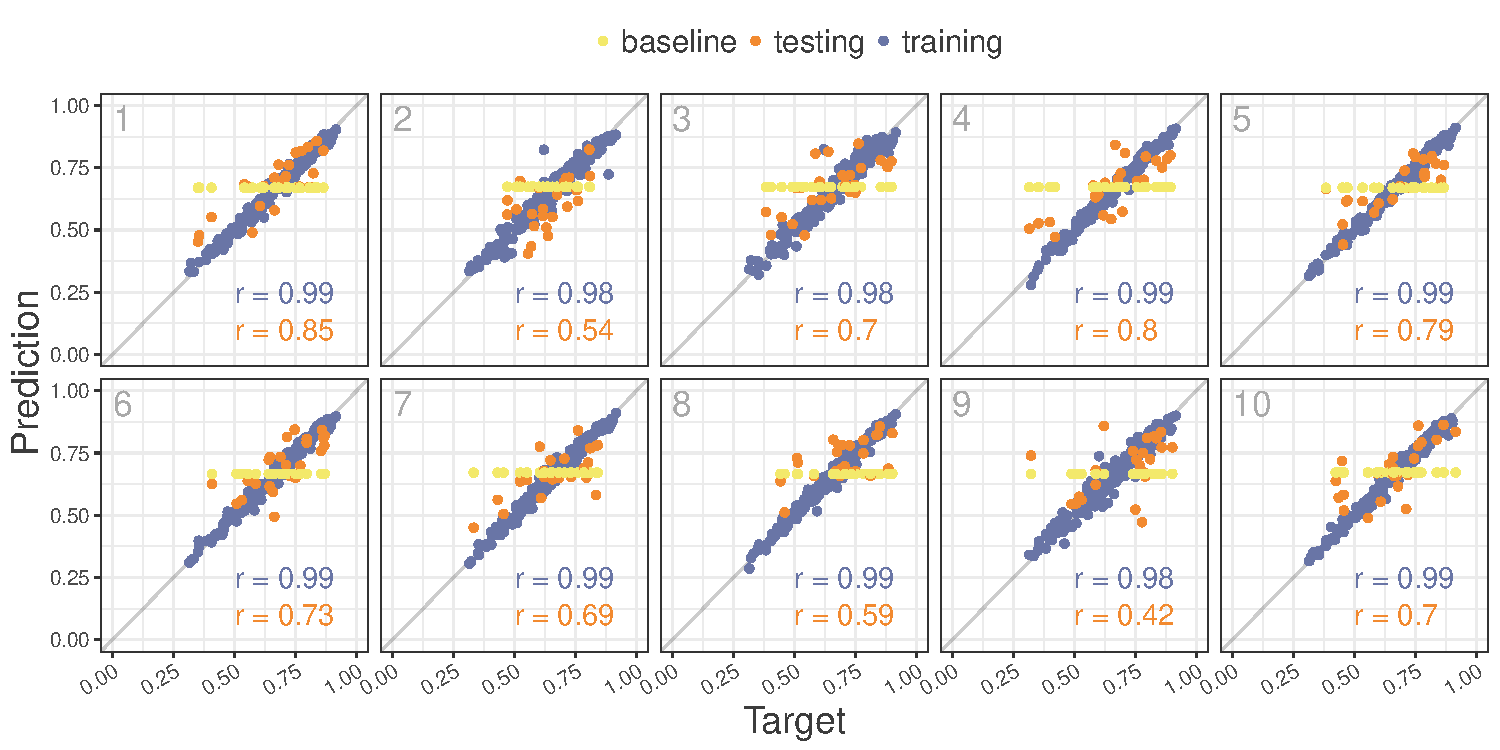
\includegraphics[width=\linewidth]{graphs/all-pred-target-epoch30.pdf}
	\caption{Testing label (x axis) vs. model prediction (y axis) after training; faceted over cross-validation configurations.}
	\label{fig:app-corr-posttraining}
\end{figure*}

\end{document}
